%%%%%%%%%%%%%%%%%%%%%%%%%%%%%%%%%%%%%
%                                   %
% Compile with XeLaTeX and biber    %
%                                   %
% Questions or comments:            %
%                                   %
% joshua dot mcneill at uga dot edu %
%                                   %
%%%%%%%%%%%%%%%%%%%%%%%%%%%%%%%%%%%%%

\documentclass{beamer}
  % Read in standard preamble (cosmetic stuff)
  %%%%%%%%%%%%%%%%%%%%%%%%%%%%%%%%%%%%%%%%%%%%%%%%%%%%%%%%%%%%%%%%
% This is a standard preamble used in for all slide documents. %
% It basically contains cosmetic settings.                     %
%                                                              %
% Joshua McNeill                                               %
% joshua dot mcneill at uga dot edu                            %
%%%%%%%%%%%%%%%%%%%%%%%%%%%%%%%%%%%%%%%%%%%%%%%%%%%%%%%%%%%%%%%%

% Beamer settings
% \usetheme{Berkeley}
\usetheme{CambridgeUS}
% \usecolortheme{dove}
% \usecolortheme{rose}
\usecolortheme{seagull}
\usefonttheme{professionalfonts}
\usefonttheme{serif}
\setbeamertemplate{bibliography item}{}

% Packages and settings
\usepackage{fontspec}
  \setmainfont{Charis SIL}
\usepackage{hyperref}
  \hypersetup{colorlinks=true,
              allcolors=blue}
\usepackage{graphicx}
  \graphicspath{{../../figures/}}
\usepackage[normalem]{ulem}
\usepackage{enumerate}

% Document information
\author{M. McNeill}
\title[FREN2001]{Français 2001}
\institute{\url{joshua.mcneill@uga.edu}}
\date{}

%% Custom commands
% Lexical items
\newcommand{\lexi}[1]{\textit{#1}}
% Gloss
\newcommand{\gloss}[1]{`#1'}
\newcommand{\tinygloss}[1]{{\tiny`#1'}}
% Orthographic representations
\newcommand{\orth}[1]{$\langle$#1$\rangle$}
% Utterances (pragmatics)
\newcommand{\uttr}[1]{`#1'}
% Sentences (pragmatics)
\newcommand{\sent}[1]{\textit{#1}}
% Base dir for definitions
\newcommand{\defs}{../definitions}


  % Packages and settings

  % Document information
  \subtitle[\lexi{Aller} et expressions temporelles]{Le verbe \lexi{aller} et les expressions temporelles}

\begin{document}
  % Read in the standard intro slides (title page and table of contents)
  \begin{frame}
    \titlepage
    \tiny{Office: % Basically a variable for office hours location
Gilbert 121\\
          Office hours: % Basically a variable for office hours
 lundi, mercredi, vendredi 10:10--11:10
}
  \end{frame}

  \begin{frame}{}
    \begin{center}
      \Large Quiz
    \end{center}
  \end{frame}

  \begin{frame}{Annonces}
    \begin{itemize}
      \item L'examen 1 est le 30 septembre (vendredi)
      \item[] \tinygloss{Exam 1 is September 30th (Friday)}
      \item Nous allons réviser mercredi
      \item[] \tinygloss{We will review Wednesday}
    \end{itemize}
  \end{frame}

  \begin{frame}{Quand?}
    \begin{columns}
      \column{0.6\textwidth}
        Est'ce que ça se passe maintenant ou plus tard?
        \begin{center}
          {\scriptsize
          \begin{tabular}{p{3cm} | c | c}
            \hline
            Activité                              & Maintenant?             & Plus tard? \\
            \hline
            1) Ils vont nager un peu.                &                         & \uncover<2->{$\times$} \\
            2) Ils vont manger.                      &                         & \uncover<4->{$\times$} \\
            3) Ils vont au gymnase.                  & \uncover<6->{$\times$}  & \\
            4) Ils vont au cinéma.                   & \uncover<8->{$\times$}  & \\
            5) Ils vont travailler toute la journée. &                         & \uncover<10->{$\times$} \\
            6) Ils vont faire de la marche.          &                         & \uncover<12->{$\times$} \\
            7) Ils vont au parc.                     & \uncover<14->{$\times$} & \\
            8) Ils vont voir un film.                &                         & \uncover<16->{$\times$} \\
            \hline
          \end{tabular}
          }
        \end{center}
      \column{0.4\textwidth}
        \begin{minipage}[c][0.6\textheight]{\linewidth}
          \begin{center}
            \only<1-2>{
              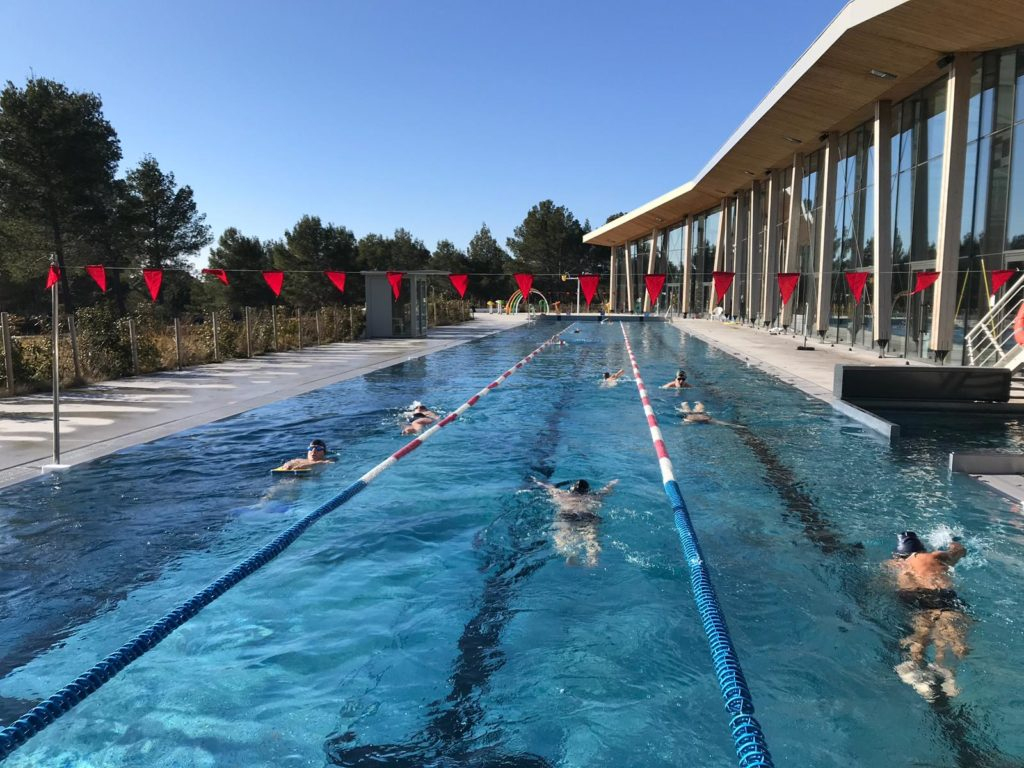
\includegraphics[scale=0.17]{piscine.jpeg}
            }
            \only<3-4>{
              
\includegraphics[scale=0.25]{manger.jpg}
            }
            \only<5-6>{
              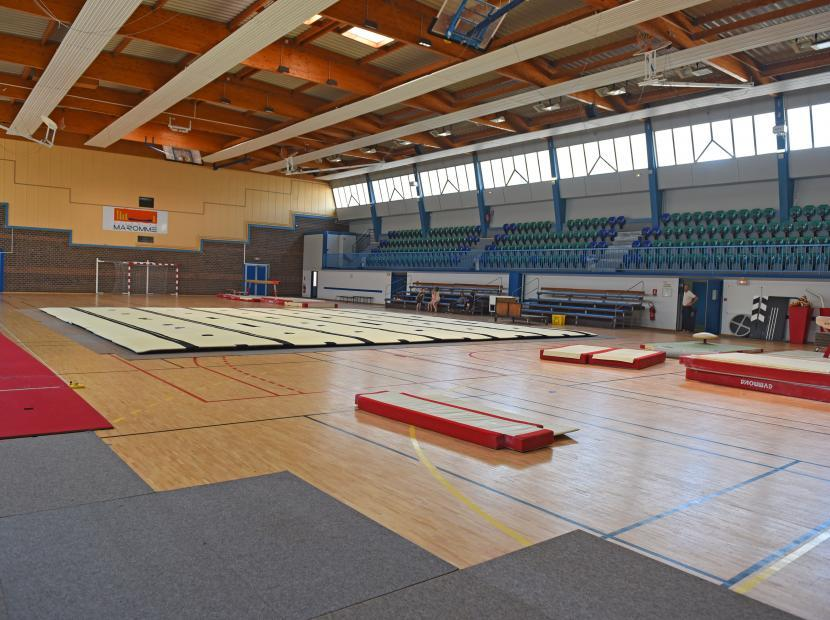
\includegraphics[scale=0.16]{gymnase.jpg}
            }
            \only<7-8>{
              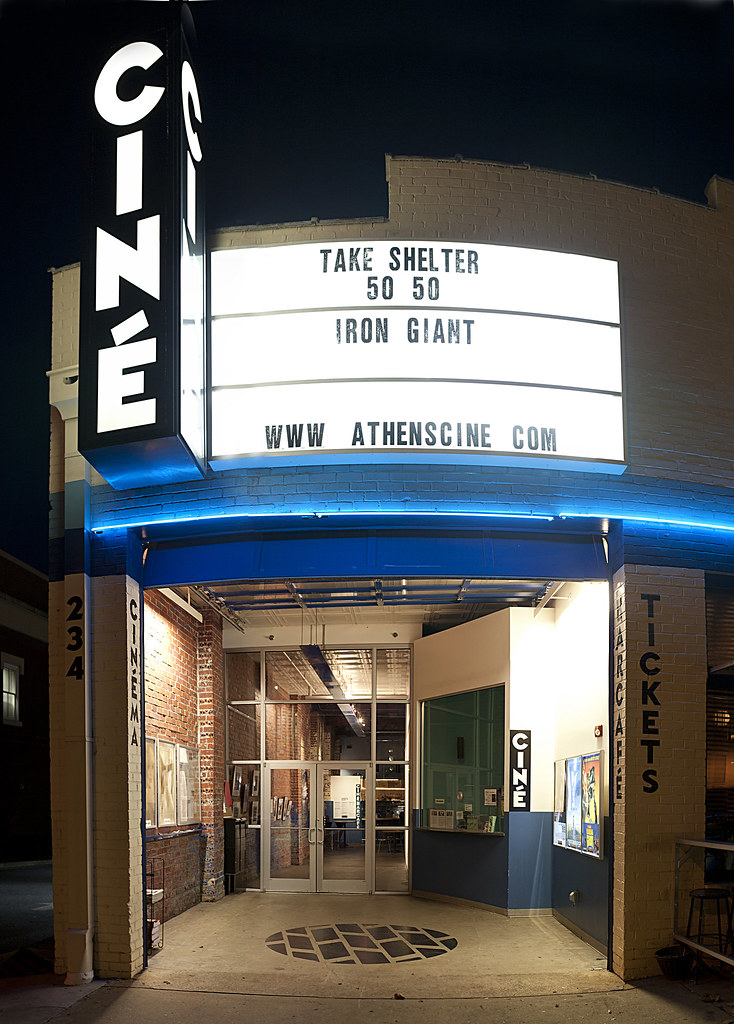
\includegraphics[scale=0.15]{cine.jpg}
            }
            \only<9-10>{
              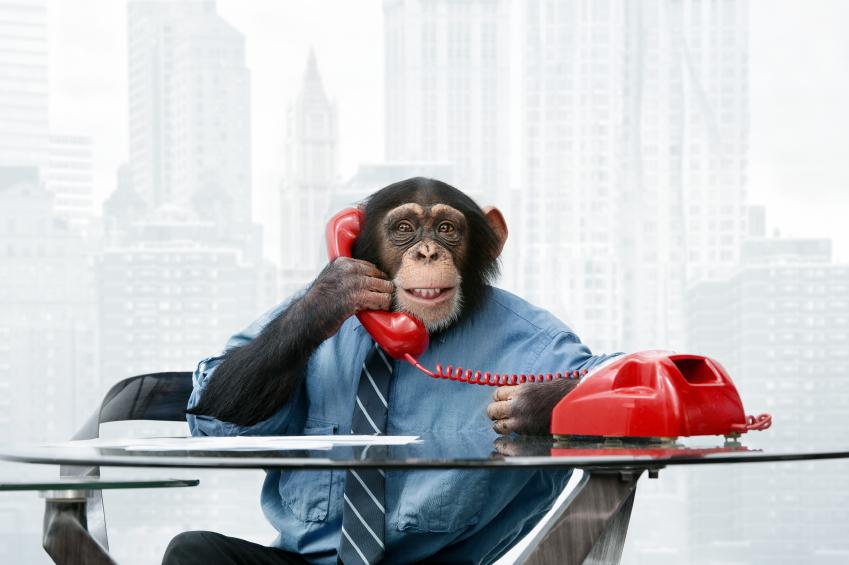
\includegraphics[scale=0.5]{travailler.jpg}
            }
            \only<11-12>{
              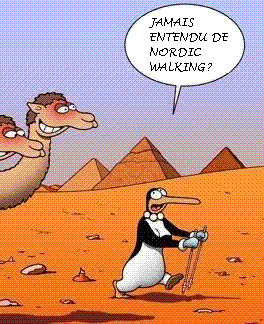
\includegraphics[scale=0.45]{marche.jpg}
            }
            \only<13-14>{
              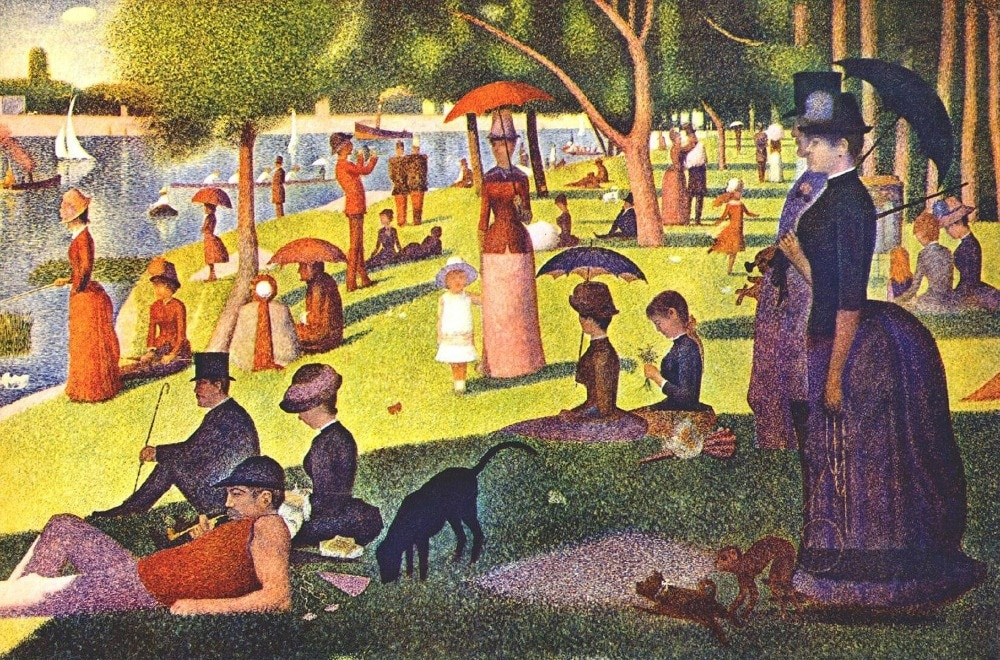
\includegraphics[scale=0.14]{dimanche_parc.jpg} \\
              \lexi{Un dimanche après-midi à l'Île de la Grande Jatte} par Georges Seurat (1884-1886)
            }
            \only<15-16>{
              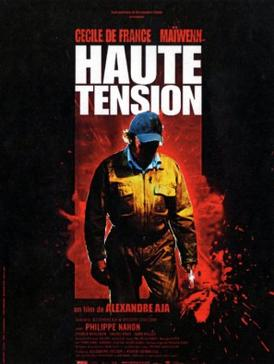
\includegraphics[scale=0.4]{haute_tension.jpg}
            }
          \end{center}
        \end{minipage}
    \end{columns}
  \end{frame}

  \begin{frame}{Vos projets}
    Demandez à un partenaire quels sont ses projets aux moments suivants.
    Rapportez une réponse à la classe. \\
    \tinygloss{Ask a partner what their plans are for the following times.
    Report an answer to the class.}
    \begin{columns}
      \column{0.5\textwidth}
        \begin{description}
          \item[] \textbf{Modèle:}
          \item[] \emph{cet après-midi}
          \item[E1:] Qu'est-ce que tu vas faire cet après-midi?
          \item[E2:] Cet après-midi, je vais travailler. Et toi?
          \item[E1:] Mon ami et moi, nous allons jouer au tennis.
        \end{description}
      \column{0.5\textwidth}
        \begin{enumerate}
          \item ce soir
          \item demain
          \item ce week-end
          \item l'été prochain
        \end{enumerate}
    \end{columns}
  \end{frame}

  \begin{frame}{}
    \begin{center}
      \Large Questions?
    \end{center}
  \end{frame}
\end{document}
